\documentclass[conference]{IEEEtran}
\IEEEoverridecommandlockouts

\usepackage{cite}
\usepackage{amsmath,amssymb,amsfonts}
\usepackage{algorithmic}
\usepackage{graphicx}
\usepackage{textcomp}
\usepackage{xcolor}
\usepackage{booktabs}
\usepackage{multirow}
\usepackage{url}

\graphicspath{{../results/figures/}}

\begin{document}

\title{Noise-Aware Hybrid Quantum-Classical Graph Neural Networks for Out-of-Distribution Molecular Property Prediction Under Bemis--Murcko Scaffold Splitting}

\author{\IEEEauthorblockN{[Author Name(s)]}
\IEEEauthorblockA{\textit{[Department]} \\
\textit{[Institution]}\\
[City, Country] \\
[Email Address]}
}

\maketitle

\begin{abstract}
Predicting absorption, distribution, metabolism, excretion, and toxicity (ADMET) properties on novel chemical scaffolds remains a central bottleneck in computational drug discovery. Existing hybrid quantum-classical graph neural networks (QGNNs) often report inflated accuracy due to random train/test data leakage, omit parameter-matched classical baselines, and lack validation on Noisy Intermediate-Scale Quantum (NISQ) hardware. We present a reproducible, noise-aware Hybrid QGNN framework evaluated under strict deterministic 80/10/10 Bemis--Murcko scaffold splitting on MoleculeNet BBBP ($N=2{,}039$) and BACE ($N=1{,}513$). A 3-layer \texttt{GINEConv} encoder (42,500 parameters) compresses 45-dimensional atom and 12-dimensional bond graphs into a 4-dimensional $[-\pi,\pi]$ latent vector fed into a 4-qubit, 3-layer variational quantum circuit (41 head parameters: 36 circuit weights plus a $4\rightarrow 1$ linear readout), benchmarked against an exact 41-parameter classical MLP baseline. Under scaffold splitting on BACE, the Hybrid QGNN achieves $0.8340 \pm 0.0280$ Test ROC-AUC and $0.7455 \pm 0.0275$ PR-AUC (versus $0.8360 \pm 0.0031$ ROC-AUC and $0.7168 \pm 0.0267$ PR-AUC for the parameter-matched classical baseline), while random splitting inflates BBBP ROC-AUC by $+0.1921$. On PennyLane's \texttt{default.mixed} simulator, Zero-Noise Extrapolation (ZNE) reduces Pauli-$Z$ expectation MAE by up to $71\%$. Finally, a single batched \texttt{EstimatorV2} job on IBM's \texttt{ibm\_fez} QPU (Job ID \texttt{dc3q0pls2omc738e1m2g}, $N=50$) achieves $0.8981$ ROC-AUC versus $0.9002$ ideal simulation ($\text{MAE}=0.0677$).
\end{abstract}

\begin{IEEEkeywords}
Quantum Machine Learning, Graph Neural Networks, Drug Discovery, ADMET, Bemis--Murcko Scaffold Split, Zero-Noise Extrapolation, IBM Quantum.
\end{IEEEkeywords}

\section{Introduction}
More than 90\% of drug candidates fail during clinical development, frequently due to poor ADMET profiles or inability to cross the blood--brain barrier (BBB) for central nervous system (CNS) indications \cite{martins2012bayesian,molsurvey2026}. Classical Graph Neural Networks (GNNs) naturally model molecules as graphs $G=(V,E)$, yet they face two persistent challenges in medicinal chemistry: (i) severe performance degradation when generalizing out-of-distribution (OOD) to unseen core ring scaffolds \cite{bemis1996properties,wu2018moleculenet}, and (ii) overfitting when labeled bioassay datasets contain only 1,500--2,000 compounds \cite{subramanian2016computational}.

Hybrid Quantum-Classical Graph Neural Networks (QGNNs) pair a classical message-passing encoder with a compact Parameterized Quantum Circuit (PQC) readout \cite{hybridqgnn2024,bergholm2018pennylane}. Rather than encoding an entire 30-atom drug directly onto qubits, the classical GNN aggregates local atomic and bond topology into a compact $n_q$-dimensional vector that drives a $n_q$-qubit variational circuit. Despite promising early results, three methodological gaps limit the scientific credibility of prior QGNN studies \cite{molsurvey2026}:
\begin{enumerate}
    \item \textbf{Random-Split Data Leakage:} Random train/test splits place close structural analogues across splits, masking OOD generalization failure.
    \item \textbf{Unfair Classical Baselines:} Quantum readouts are rarely compared against classical heads with an identical trainable parameter budget.
    \item \textbf{Simulator-Only Evaluation:} Most studies omit density-matrix noise sweeps, error mitigation, and real quantum processing unit (QPU) execution.
\end{enumerate}

In this work, we address all three gaps on MoleculeNet BBBP and BACE \cite{wu2018moleculenet} with: (1) strict deterministic 80/10/10 Bemis--Murcko scaffold splitting with verified zero scaffold overlap; (2) an exact 41-parameter head parity comparison between angle-encoded/data-reuploading PQCs and a parameter-matched classical MLP; and (3) density-matrix NISQ noise + Zero-Noise Extrapolation (ZNE) sweeps alongside real IBM Quantum (\texttt{ibm\_fez}) hardware validation.

\section{Related Work}
\subsection{Molecular Graph Neural Networks and Scaffold Splitting}
Message-passing architectures such as \texttt{GINEConv} \cite{hu2020strategies} incorporate both atom and bond attributes, making them strong baselines on MoleculeNet benchmarks \cite{wu2018moleculenet}. However, recent surveys emphasize that random splitting overestimates real-world hit-discovery accuracy, whereas Bemis--Murcko scaffold decomposition \cite{bemis1996properties} enforces genuine OOD evaluation on unseen molecular frameworks \cite{molsurvey2026}.

\subsection{Hybrid Quantum-Classical ML and NISQ Mitigation}
Variational quantum classifiers using angle embedding and \texttt{StronglyEntanglingLayers} \cite{schuld2020circuit}, as well as data re-uploading architectures \cite{perez2020data}, can be trained end-to-end with PyTorch via PennyLane's \texttt{TorchLayer} \cite{bergholm2018pennylane}. On current NISQ devices, gate depolarizing noise and readout errors attenuate expectation values, motivating lightweight mitigation such as digital Zero-Noise Extrapolation (ZNE) via unitary folding \cite{temme2017error,giurgica2020digital}.

\section{Methodology}
\subsection{RDKit Graph Featurization and Bemis--Murcko Splitting}
Each SMILES string is parsed with RDKit into a PyTorch Geometric graph $G=(V,E)$ with $d_v = 45$ node features (one-hot atomic symbol, degree, formal charge, hybridization, aromaticity, total hydrogens, ring membership, and chirality) and $d_e = 12$ edge features (one-hot bond type, conjugation, ring membership, and stereo). Invalid SMILES are logged and excluded (11 in BBBP, yielding $N=2{,}039$; 0 in BACE, $N=1{,}513$).

For OOD evaluation, we compute canonical Murcko scaffolds (\texttt{includeChirality=False}) \cite{bemis1996properties}, sort scaffold groups largest-first (tie-breaking deterministically by scaffold SMILES), and assign whole groups to Train (80\%), Validation (10\%), and Test (10\%) splits. We assert $\mathcal{S}_{\text{train}} \cap \mathcal{S}_{\text{val}} = \mathcal{S}_{\text{train}} \cap \mathcal{S}_{\text{test}} = \mathcal{S}_{\text{val}} \cap \mathcal{S}_{\text{test}} = \emptyset$.

\subsection{Classical GNN Encoder and Parameter-Matched Baseline}
Our shared \texttt{MolecularGNNEncoder} projects node and edge features to $h=64$ dimensions, applies 3 residual \texttt{GINEConv} layers with \texttt{BatchNorm1d}, \texttt{ReLU}, and \texttt{Dropout(0.2)}, concatenates \texttt{global\_mean\_pool} and \texttt{global\_max\_pool} ($128$-D), and projects to $n_q$ latent angles bounded strictly to $[-\pi, \pi]$:
\begin{equation}
\mathbf{z} = \pi \tanh\!\left(\mathbf{W}_{\text{bot}} \left[\mathbf{h}_{\text{mean}} \,\|\, \mathbf{h}_{\text{max}}\right] + \mathbf{b}_{\text{bot}}\right) \in [-\pi, \pi]^{n_q}.
\end{equation}
The encoder contains $42{,}500$ trainable parameters for $n_q=4$. We compare two classical baselines: \texttt{ClassicalGNNFull} (2-layer MLP, $4 \rightarrow 32 \rightarrow 1$, $193$ head parameters) and \texttt{ClassicalGNNParamMatched} (bias-free $4 \rightarrow 8$ linear layer + \texttt{ReLU} + $8 \rightarrow 1$ linear layer, $4\times 8 + 8\times 1 + 1 = 41$ head parameters).

\subsection{Variational Quantum Readout and Hybrid QGNN}
The \texttt{QuantumReadoutLayer} prepares $|0\rangle^{\otimes n_q}$ and evaluates two ans\"{a}tze with identical weight tensor $\boldsymbol{\theta} \in \mathbb{R}^{L \times n_q \times 3}$ ($3 n_q L = 36$ weights for $n_q=4, L=3$):
\begin{itemize}
    \item \textbf{Angle Encoding (\texttt{hybrid\_angle}):} A single $R_Y(z_i)$ embedding layer followed by $L$ layers of \texttt{StronglyEntanglingLayers} (single-qubit $R_Z(\omega)R_Y(\theta)R_Z(\phi)$ rotations and cyclic \texttt{CNOT} entanglement with range $r = (l \bmod (n_q-1)) + 1$).
    \item \textbf{Data Re-Uploading (\texttt{hybrid\_reuploading}):} Re-applies $R_Y(z_i)$ before each of the $L$ entangling blocks.
\end{itemize}
Measuring $\hat{e}_i = \langle \psi(\mathbf{z}, \boldsymbol{\theta}) | Z_i | \psi(\mathbf{z}, \boldsymbol{\theta}) \rangle \in [-1, 1]$ for $i \in \{0,\dots,n_q-1\}$ yields $\hat{\mathbf{e}} \in \mathbb{R}^{n_q}$, followed by a classical linear head $\hat{y} = \mathbf{w}^\top \hat{\mathbf{e}} + b$ ($4+1=5$ parameters), totaling $41$ head parameters ($42{,}541$ total). Fig.~\ref{fig:circuits} illustrates both 4-qubit circuits.

\begin{figure}[t]
\centering
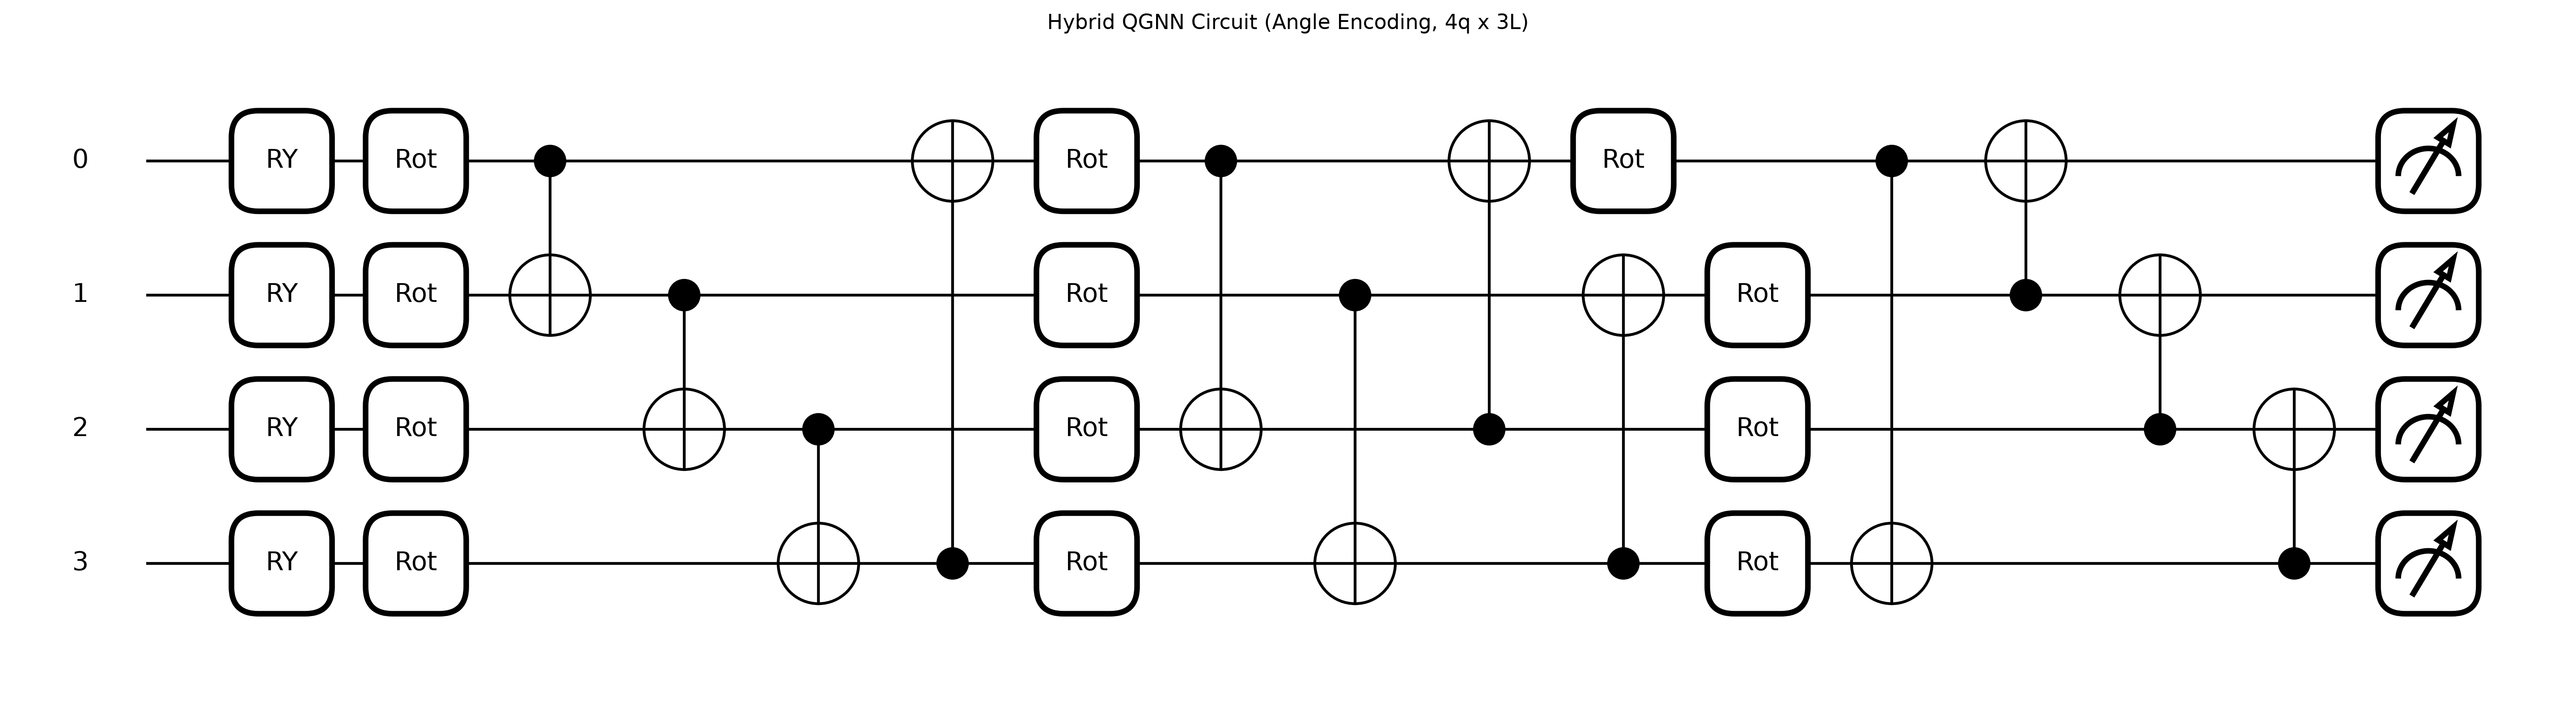
\includegraphics[width=\linewidth]{circuit_angle_4q3l.png}
\vspace{2pt}
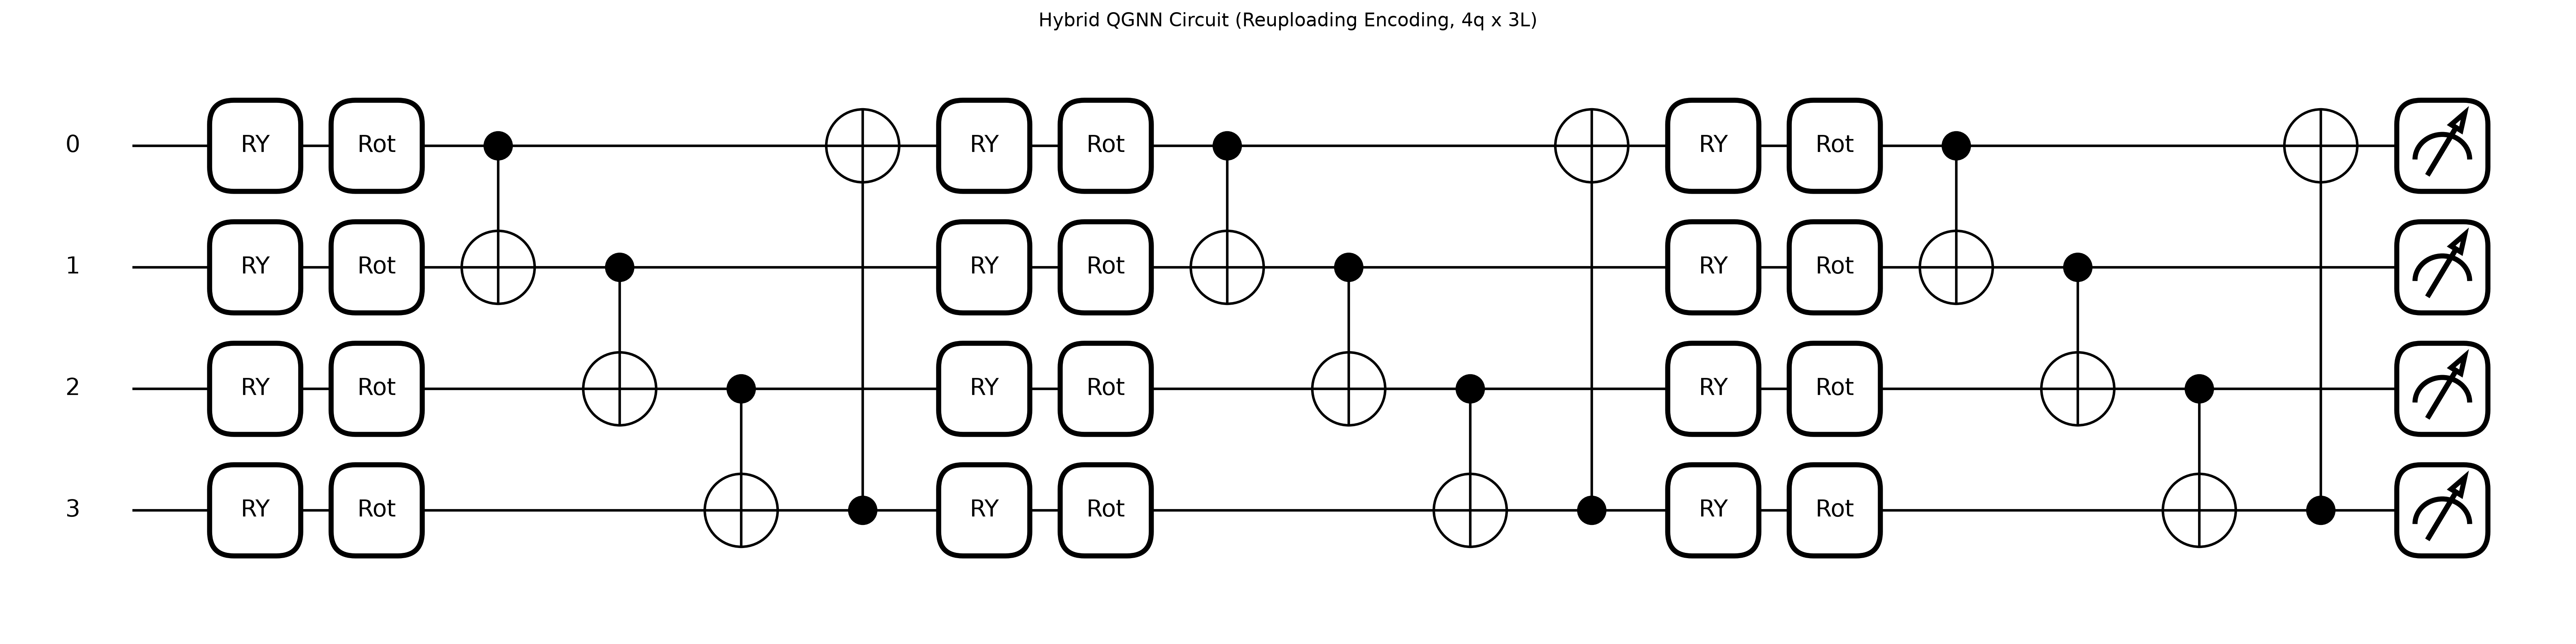
\includegraphics[width=\linewidth]{circuit_reuploading_4q3l.png}
\caption{Top: 4-qubit $\times$ 3-layer \texttt{hybrid\_angle} circuit (12 \texttt{CNOT}s, depth 14). Bottom: \texttt{hybrid\_reuploading} circuit with identical 36 variational parameters.}
\label{fig:circuits}
\end{figure}

\subsection{Training Objective and Zero-Noise Extrapolation (ZNE)}
Models are trained with \texttt{BCEWithLogitsLoss} using train-split positive class weighting $w_+ = N_{\text{neg}} / N_{\text{pos}}$, \texttt{AdamW} ($\text{lr}=10^{-3}$, weight decay $10^{-4}$), cosine annealing, gradient clipping ($\|\nabla\|_2 \le 1.0$), and early stopping on Validation ROC-AUC (patience 20, max 100 epochs).

For NISQ error mitigation, we apply digital unitary folding $U \mapsto U U^\dagger U$ (noise scale factor $s=3$) alongside the unmitigated circuit ($s=1$) on PennyLane's \texttt{default.mixed} simulator with gate depolarizing noise $p$ and readout \texttt{BitFlip} ($p_{\text{ro}}=0.01$ for $p>0$). Linear Richardson extrapolation estimates the zero-noise expectation value:
\begin{equation}
\hat{e}_{i,\text{ZNE}} = \operatorname{clip}\!\left(\frac{3\,\hat{e}_{i}^{(s=1)} - \hat{e}_{i}^{(s=3)}}{2},\, -1,\, 1\right).
\end{equation}

\section{Experimental Setup}
Table~\ref{tab:splits} summarizes the deterministic scaffold splits. Main experiments run across 5 fixed seeds $\{42,43,44,45,46\}$ on an NVIDIA RTX 3050 Laptop GPU with PennyLane \texttt{default.qubit} (\texttt{diff\_method="backprop"}). Ablation sweeps use 5 seeds for classical runs and 3 seeds $\{42,43,44\}$ for quantum sweeps.

\begin{table}[t]
\centering
\caption{Deterministic 80/10/10 Bemis--Murcko Scaffold Splits}
\label{tab:splits}
\begin{tabular}{@{}lcccc@{}}
\toprule
Dataset & Split & Molecules & Scaffolds & Pos. Ratio \\
\midrule
\multirow{3}{*}{BBBP ($N=2{,}039$)} & Train & 1,631 & 617 & 0.7474 \\
 & Val & 204 & 204 & 0.7843 \\
 & Test & 204 & 204 & 0.8873 \\
\midrule
\multirow{3}{*}{BACE ($N=1{,}513$)} & Train & 1,210 & 368 & 0.4843 \\
 & Val & 151 & 151 & 0.4238 \\
 & Test & 152 & 152 & 0.2697 \\
\bottomrule
\end{tabular}
\end{table}

For real hardware validation, we select the best validation-AUC BACE \texttt{hybrid\_angle} checkpoint (\texttt{seed=42}, $\text{Val ROC-AUC}=0.8396$), extract 4-D latent vectors for a stratified 50-molecule test subset (13 positives, 26.0\%), verify local Qiskit \texttt{Statevector} equivalence ($\max |\Delta \langle Z\rangle| = 1.266 \times 10^{-7} < 10^{-5}$), transpile at \texttt{optimization\_level=3} for IBM's \texttt{ibm\_fez} QPU, and submit a single batched \texttt{EstimatorV2} job (\texttt{default\_shots=1024}).

\section{Results and Ablation Analysis}
\subsection{Main Scaffold-Split Benchmark (5 Seeds)}
Table~\ref{tab:main} reports 5-seed Mean $\pm$ Std test performance under strict scaffold splitting. On BACE, \texttt{hybrid\_angle} ($0.8340 \pm 0.0280$ ROC-AUC) achieves statistical parity with \texttt{classical\_matched} ($0.8360 \pm 0.0031$; paired $t$-test $p=0.8711$, Wilcoxon $p=0.8125$) while attaining the highest Test PR-AUC ($0.7455 \pm 0.0275$ vs.\ $0.7168 \pm 0.0267$). On BBBP, where the test split exhibits strong positive skew ($88.7\%$ permeable), \texttt{hybrid\_angle} achieves the highest Test F1 ($0.9103 \pm 0.0185$), whereas \texttt{classical\_matched} leads in ROC-AUC ($0.7479$ vs.\ $0.6928$, $p=0.0076$).

\begin{table*}[t]
\centering
\caption{5-Seed Test Performance Under Strict Bemis--Murcko Scaffold Splitting (Mean $\pm$ Std)}
\label{tab:main}
\begin{tabular}{@{}llccccc@{}}
\toprule
Dataset & Model & Head / Total Params & Test ROC-AUC & Test PR-AUC & Test F1 \\
\midrule
\multirow{4}{*}{BBBP} & \texttt{classical\_full} & 193 / 42,693 & $0.7547 \pm 0.0535$ & $0.9621 \pm 0.0109$ & $0.8840 \pm 0.0531$ \\
 & \texttt{classical\_matched} & 41 / 42,541 & $0.7479 \pm 0.0434$ & $0.9595 \pm 0.0120$ & $0.9007 \pm 0.0378$ \\
 & \texttt{hybrid\_angle} & 41 / 42,541 & $0.6928 \pm 0.0235$ & $0.9316 \pm 0.0153$ & $\mathbf{0.9103 \pm 0.0185}$ \\
 & \texttt{hybrid\_reuploading} & 41 / 42,541 & $0.6735 \pm 0.0666$ & $0.9381 \pm 0.0169$ & $0.8718 \pm 0.0411$ \\
\midrule
\multirow{4}{*}{BACE} & \texttt{classical\_full} & 193 / 42,693 & $0.8410 \pm 0.0119$ & $0.7286 \pm 0.0293$ & $0.6493 \pm 0.0388$ \\
 & \texttt{classical\_matched} & 41 / 42,541 & $0.8360 \pm 0.0031$ & $0.7168 \pm 0.0267$ & $0.6566 \pm 0.0282$ \\
 & \texttt{hybrid\_angle} & 41 / 42,541 & $0.8340 \pm 0.0280$ & $\mathbf{0.7455 \pm 0.0275}$ & $0.6563 \pm 0.0306$ \\
 & \texttt{hybrid\_reuploading} & 41 / 42,541 & $0.7800 \pm 0.1045$ & $0.6689 \pm 0.1329$ & $0.5960 \pm 0.1279$ \\
\bottomrule
\end{tabular}
\end{table*}

\subsection{Ablation A: Random vs.\ Scaffold Split Leakage}
Table~\ref{tab:ablation_a} and Fig.~\ref{fig:split_leakage} quantify the optimism bias of random splitting. On BBBP, random splitting inflates ROC-AUC by $+0.1581$ for \texttt{classical\_matched} ($0.7479 \rightarrow 0.9061$) and $+0.1921$ for \texttt{hybrid\_angle} ($0.6928 \rightarrow 0.8848$), confirming that random splits mask OOD scaffold generalization.

\begin{table}[t]
\centering
\caption{Ablation A: Random vs.\ Bemis--Murcko Scaffold Split}
\label{tab:ablation_a}
\begin{tabular}{@{}llccc@{}}
\toprule
Dataset & Model & Split (Seeds) & Test ROC-AUC & Test PR-AUC \\
\midrule
\multirow{4}{*}{BBBP} & \texttt{classical\_matched} & Scaffold (5) & $0.7479 \pm 0.0434$ & $0.9595 \pm 0.0120$ \\
 & \texttt{classical\_matched} & Random (5) & $0.9061 \pm 0.0283$ & $0.9651 \pm 0.0177$ \\
 & \texttt{hybrid\_angle} & Scaffold (5) & $0.6928 \pm 0.0235$ & $0.9316 \pm 0.0153$ \\
 & \texttt{hybrid\_angle} & Random (3) & $0.8848 \pm 0.0676$ & $0.9568 \pm 0.0304$ \\
\midrule
\multirow{4}{*}{BACE} & \texttt{classical\_matched} & Scaffold (5) & $0.8360 \pm 0.0031$ & $0.7168 \pm 0.0267$ \\
 & \texttt{classical\_matched} & Random (5) & $0.8738 \pm 0.0221$ & $0.8231 \pm 0.0472$ \\
 & \texttt{hybrid\_angle} & Scaffold (5) & $0.8340 \pm 0.0280$ & $0.7455 \pm 0.0275$ \\
 & \texttt{hybrid\_angle} & Random (3) & $0.8678 \pm 0.0316$ & $0.8059 \pm 0.0918$ \\
\bottomrule
\end{tabular}
\end{table}

\begin{figure}[t]
\centering
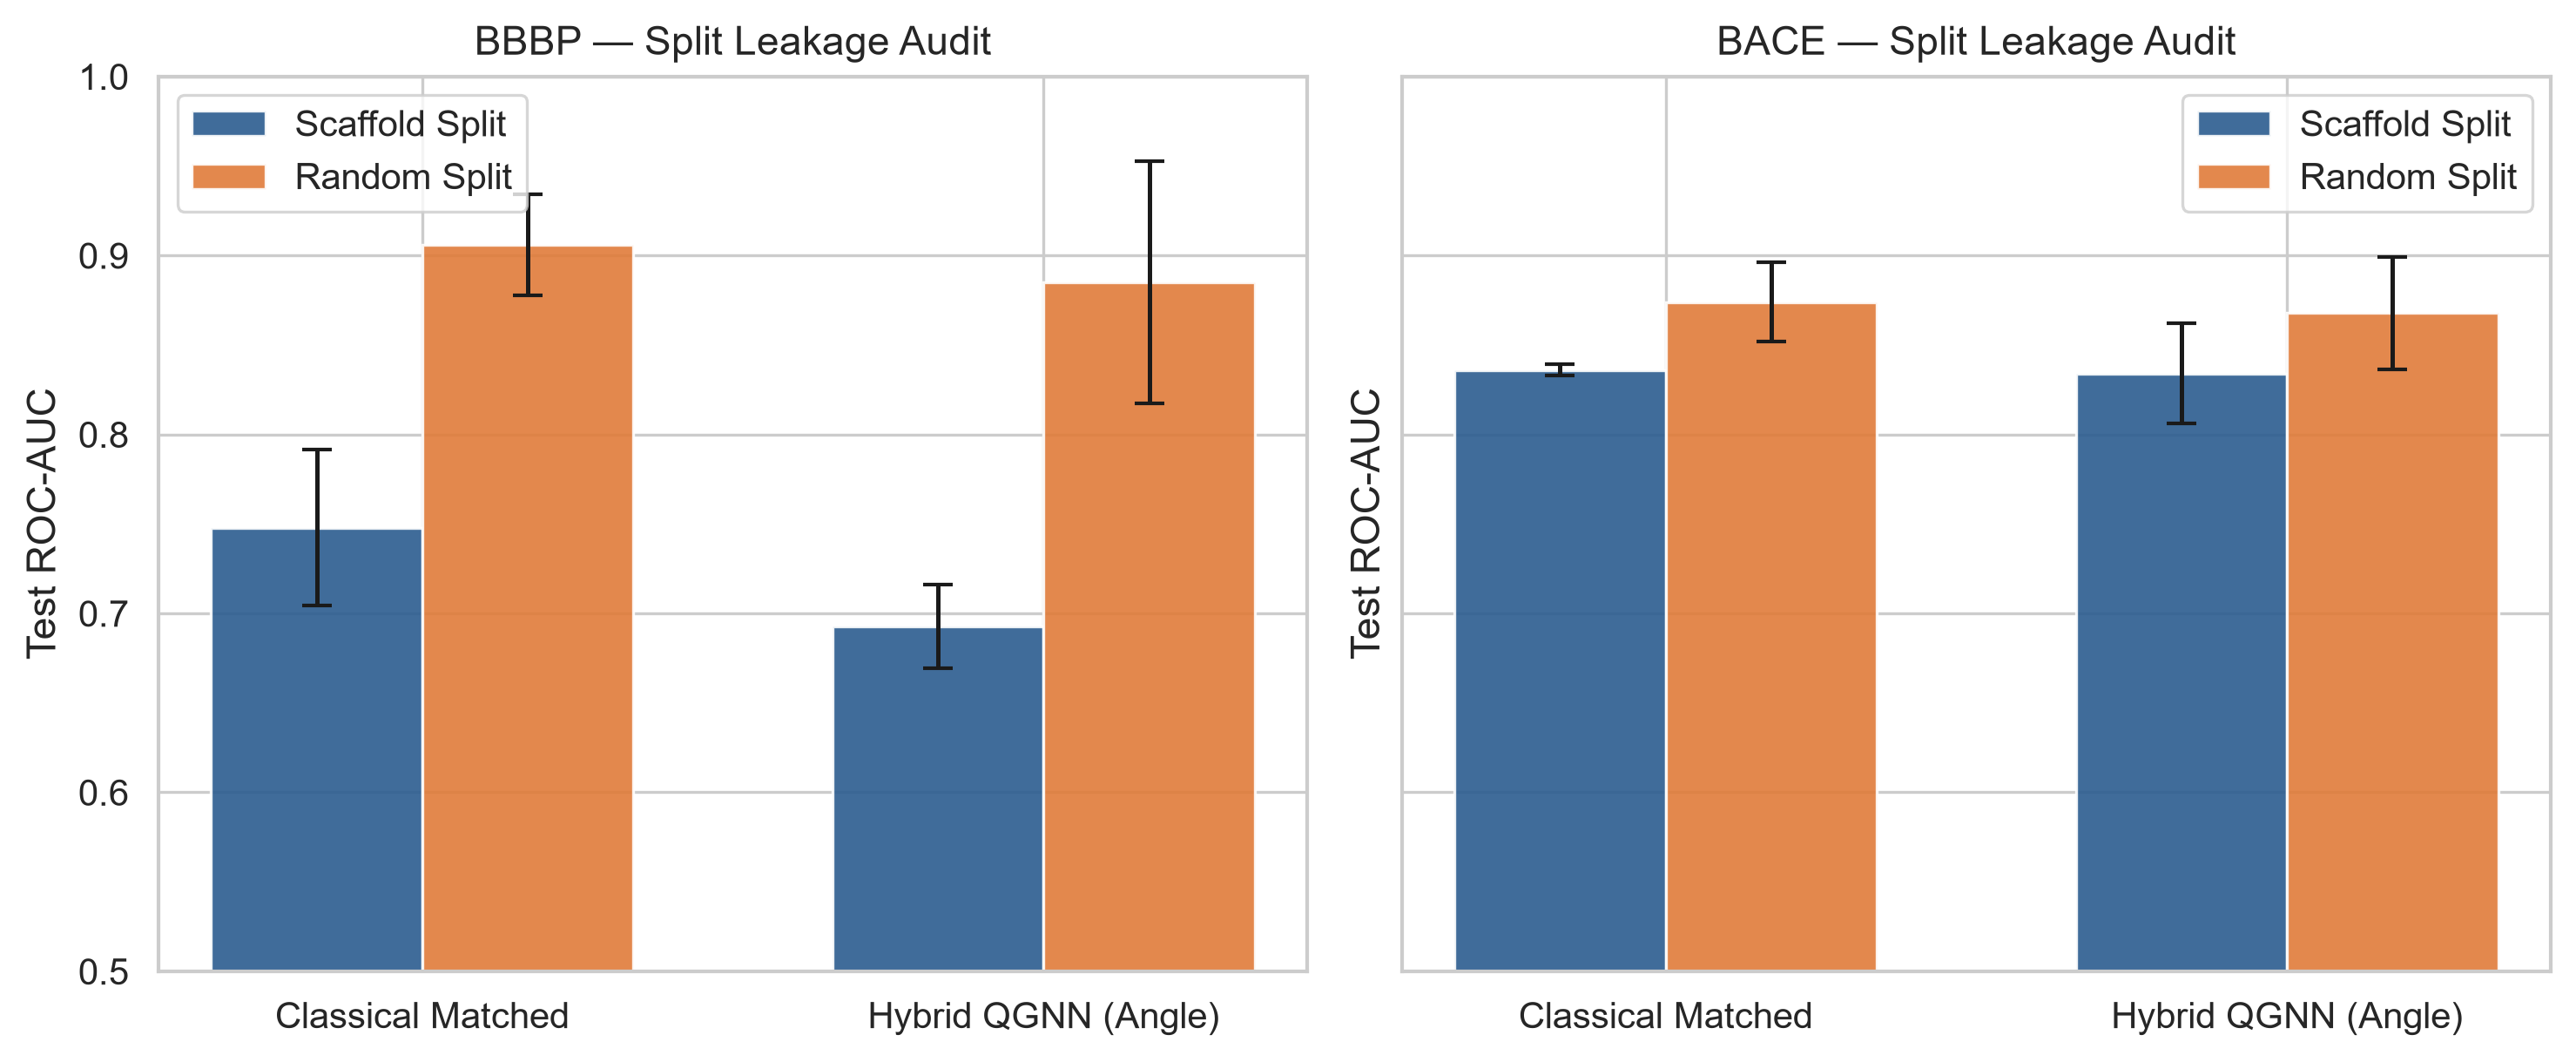
\includegraphics[width=\linewidth]{ablation_split_leakage.png}
\caption{Random vs.\ Bemis--Murcko scaffold split Test ROC-AUC across BBBP and BACE, illustrating substantial random-split leakage inflation.}
\label{fig:split_leakage}
\end{figure}

\subsection{Ablation B: Low-Data Pharmaceutical Regime}
Table~\ref{tab:ablation_b} and Fig.~\ref{fig:low_data} evaluate training fractions $f \in \{0.25, 0.50, 1.00\}$. On BACE at $f=0.50$ ($\approx 605$ training molecules), \texttt{hybrid\_angle} reaches $0.8370 \pm 0.0251$ ROC-AUC, slightly exceeding \texttt{classical\_matched} ($0.8236 \pm 0.0192$; $p=0.4866$). At extreme scarcity ($f=0.25$, $\approx 302$ molecules), \texttt{classical\_matched} degrades more gracefully ($0.8025$ vs.\ $0.7228$, $p=0.0004$), indicating that periodic quantum activations require sufficient gradient signal to align decision boundaries.

\begin{table}[t]
\centering
\caption{Ablation B: Low-Data Regime on Scaffold Split}
\label{tab:ablation_b}
\begin{tabular}{@{}llccc@{}}
\toprule
Dataset & Model & Frac (Seeds) & Test ROC-AUC & Test PR-AUC \\
\midrule
\multirow{6}{*}{BBBP} & \texttt{classical\_matched} & 0.25 (5) & $0.6641 \pm 0.0838$ & $0.9387 \pm 0.0218$ \\
 & \texttt{classical\_matched} & 0.50 (5) & $0.7301 \pm 0.0355$ & $0.9539 \pm 0.0103$ \\
 & \texttt{classical\_matched} & 1.00 (5) & $0.7479 \pm 0.0434$ & $0.9595 \pm 0.0120$ \\
 & \texttt{hybrid\_angle} & 0.25 (3) & $0.6615 \pm 0.0673$ & $0.9351 \pm 0.0182$ \\
 & \texttt{hybrid\_angle} & 0.50 (3) & $0.6770 \pm 0.0527$ & $0.9301 \pm 0.0211$ \\
 & \texttt{hybrid\_angle} & 1.00 (5) & $0.6928 \pm 0.0235$ & $0.9316 \pm 0.0153$ \\
\midrule
\multirow{6}{*}{BACE} & \texttt{classical\_matched} & 0.25 (5) & $0.8025 \pm 0.0245$ & $0.6037 \pm 0.0709$ \\
 & \texttt{classical\_matched} & 0.50 (5) & $0.8236 \pm 0.0192$ & $0.6967 \pm 0.0362$ \\
 & \texttt{classical\_matched} & 1.00 (5) & $0.8360 \pm 0.0031$ & $0.7168 \pm 0.0267$ \\
 & \texttt{hybrid\_angle} & 0.25 (3) & $0.7228 \pm 0.0240$ & $0.5258 \pm 0.1135$ \\
 & \texttt{hybrid\_angle} & 0.50 (3) & $0.8370 \pm 0.0251$ & $0.6944 \pm 0.0724$ \\
 & \texttt{hybrid\_angle} & 1.00 (5) & $0.8340 \pm 0.0280$ & $0.7455 \pm 0.0275$ \\
\bottomrule
\end{tabular}
\end{table}

\begin{figure}[t]
\centering
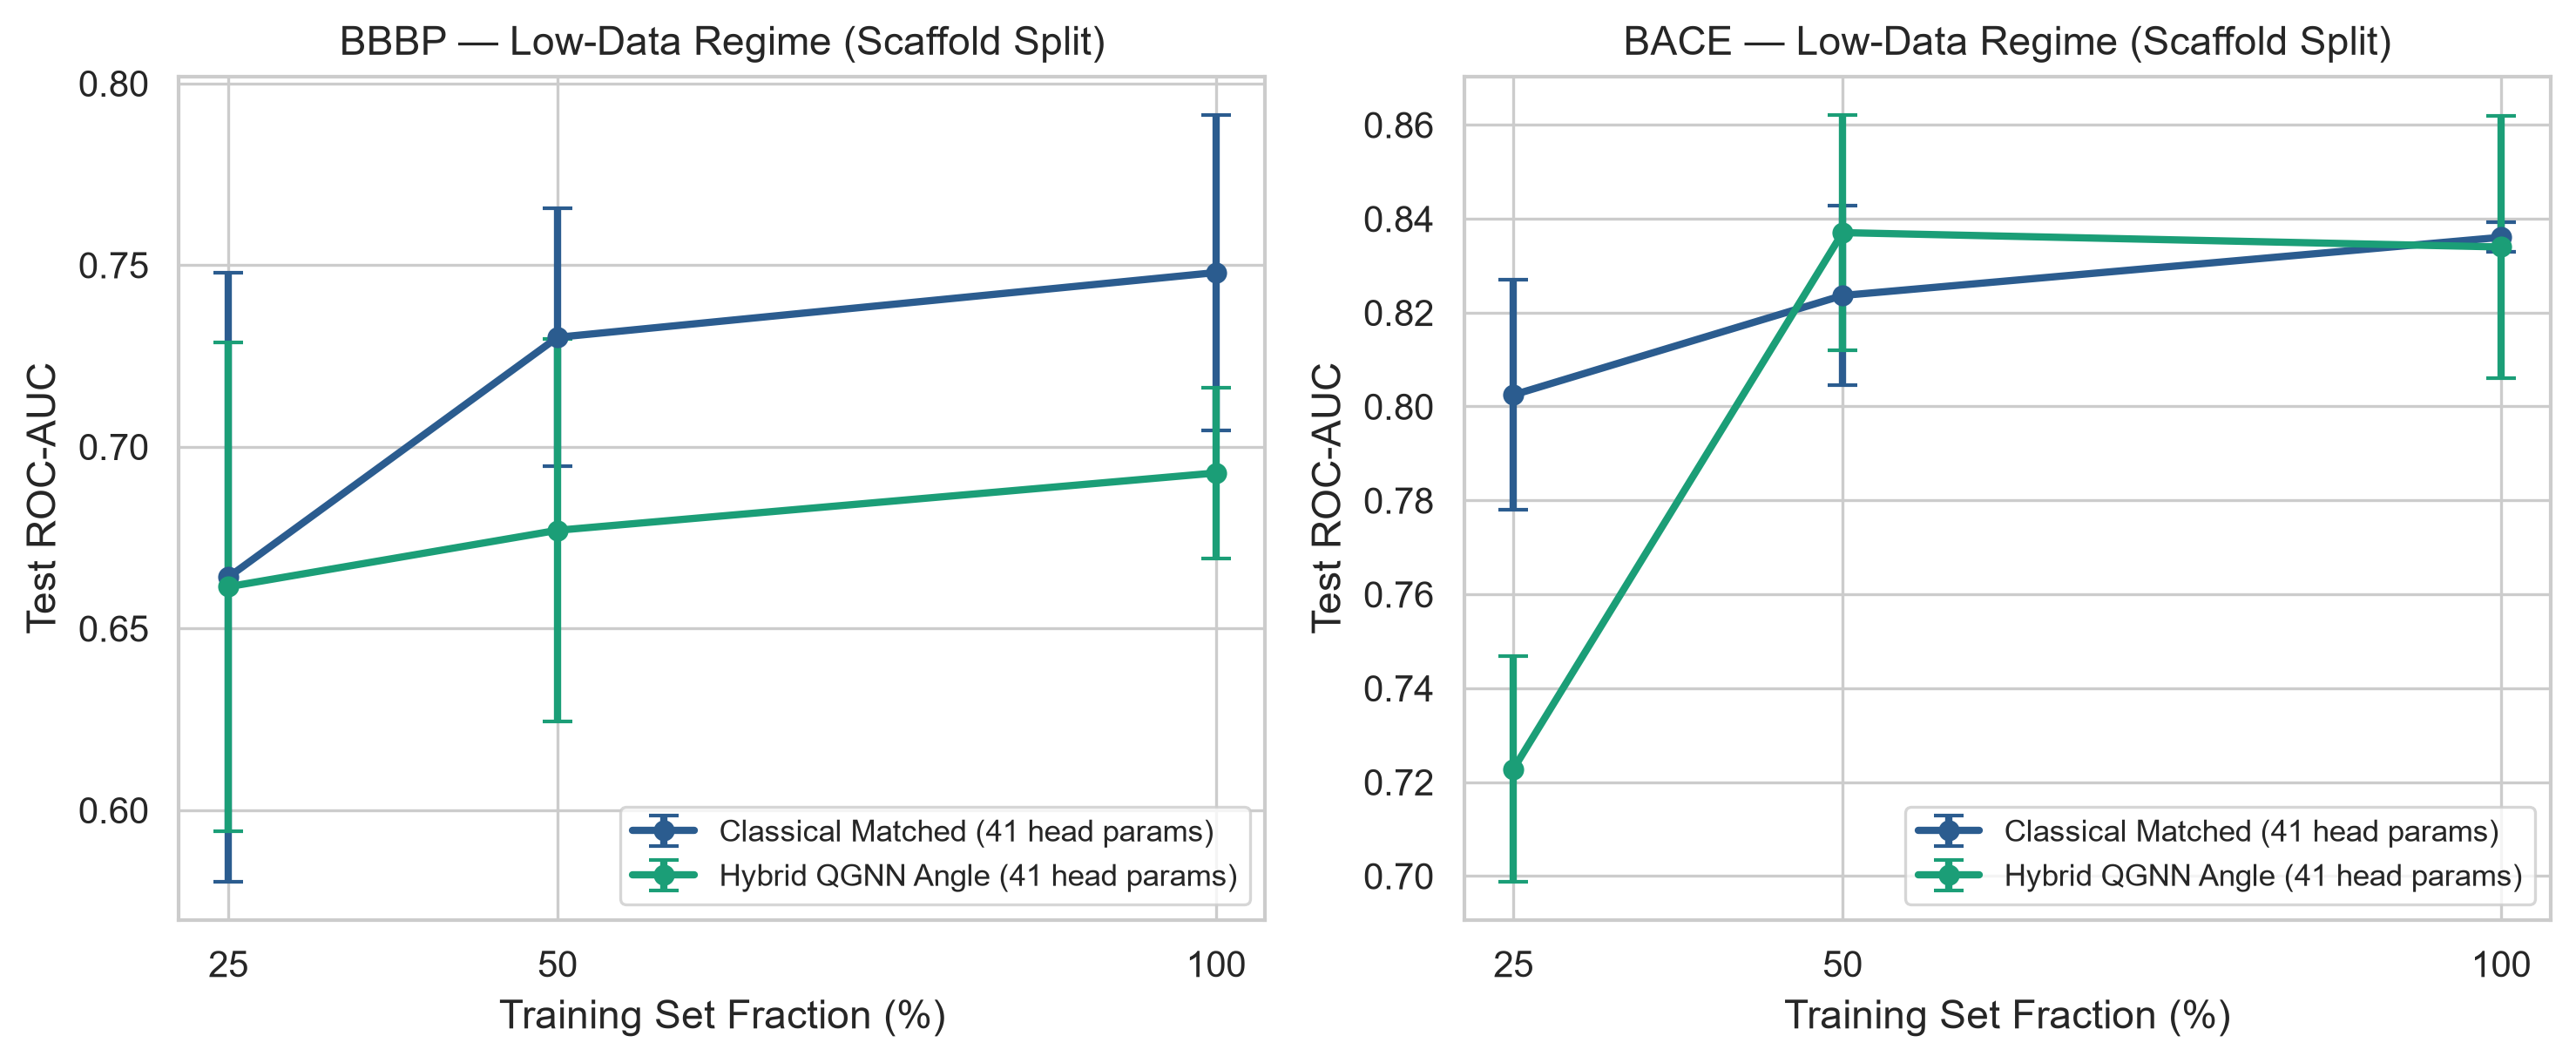
\includegraphics[width=\linewidth]{ablation_low_data.png}
\caption{Low-data learning curves (25\%, 50\%, 100\% training scaffolds) comparing \texttt{classical\_matched} and \texttt{hybrid\_angle}.}
\label{fig:low_data}
\end{figure}

\subsection{Ablation C: Qubit and Depth Sweep on BACE}
Table~\ref{tab:ablation_c} and Fig.~\ref{fig:qubit_depth} show that a shallow $4$-qubit, $1$-layer ansatz ($12$ circuit weights, $4$ \texttt{CNOT}s, depth $6$) achieves the highest BACE ROC-AUC ($0.8479 \pm 0.0134$), outperforming deeper $3$-layer circuits while minimizing NISQ gate count. Increasing to $6$ qubits ($L=3$, $18$ \texttt{CNOT}s) yields low variance ($0.8400 \pm 0.0024$) at higher circuit depth ($15$).

\begin{table}[t]
\centering
\caption{Ablation C: Qubit & Depth Sweep (BACE Scaffold Split)}
\label{tab:ablation_c}
\begin{tabular}{@{}ccccccc@{}}
\toprule
$n_q$ & $L$ & Params & CNOTs & Depth & Test ROC-AUC & Test PR-AUC \\
\midrule
4 & 1 & 12 & 4 & 6 & $\mathbf{0.8479 \pm 0.0134}$ & $0.6975 \pm 0.0850$ \\
4 & 2 & 24 & 8 & 9 & $0.8335 \pm 0.0336$ & $0.7359 \pm 0.0366$ \\
4 & 3 & 36 & 12 & 14 & $0.8340 \pm 0.0280$ & $\mathbf{0.7455 \pm 0.0275}$ \\
6 & 1 & 18 & 6 & 8 & $0.8335 \pm 0.0251$ & $0.7412 \pm 0.0448$ \\
6 & 2 & 36 & 12 & 12 & $0.8196 \pm 0.0226$ & $0.7205 \pm 0.0372$ \\
6 & 3 & 54 & 18 & 15 & $0.8400 \pm 0.0024$ & $0.7071 \pm 0.0693$ \\
\bottomrule
\end{tabular}
\end{table}

\begin{figure}[t]
\centering
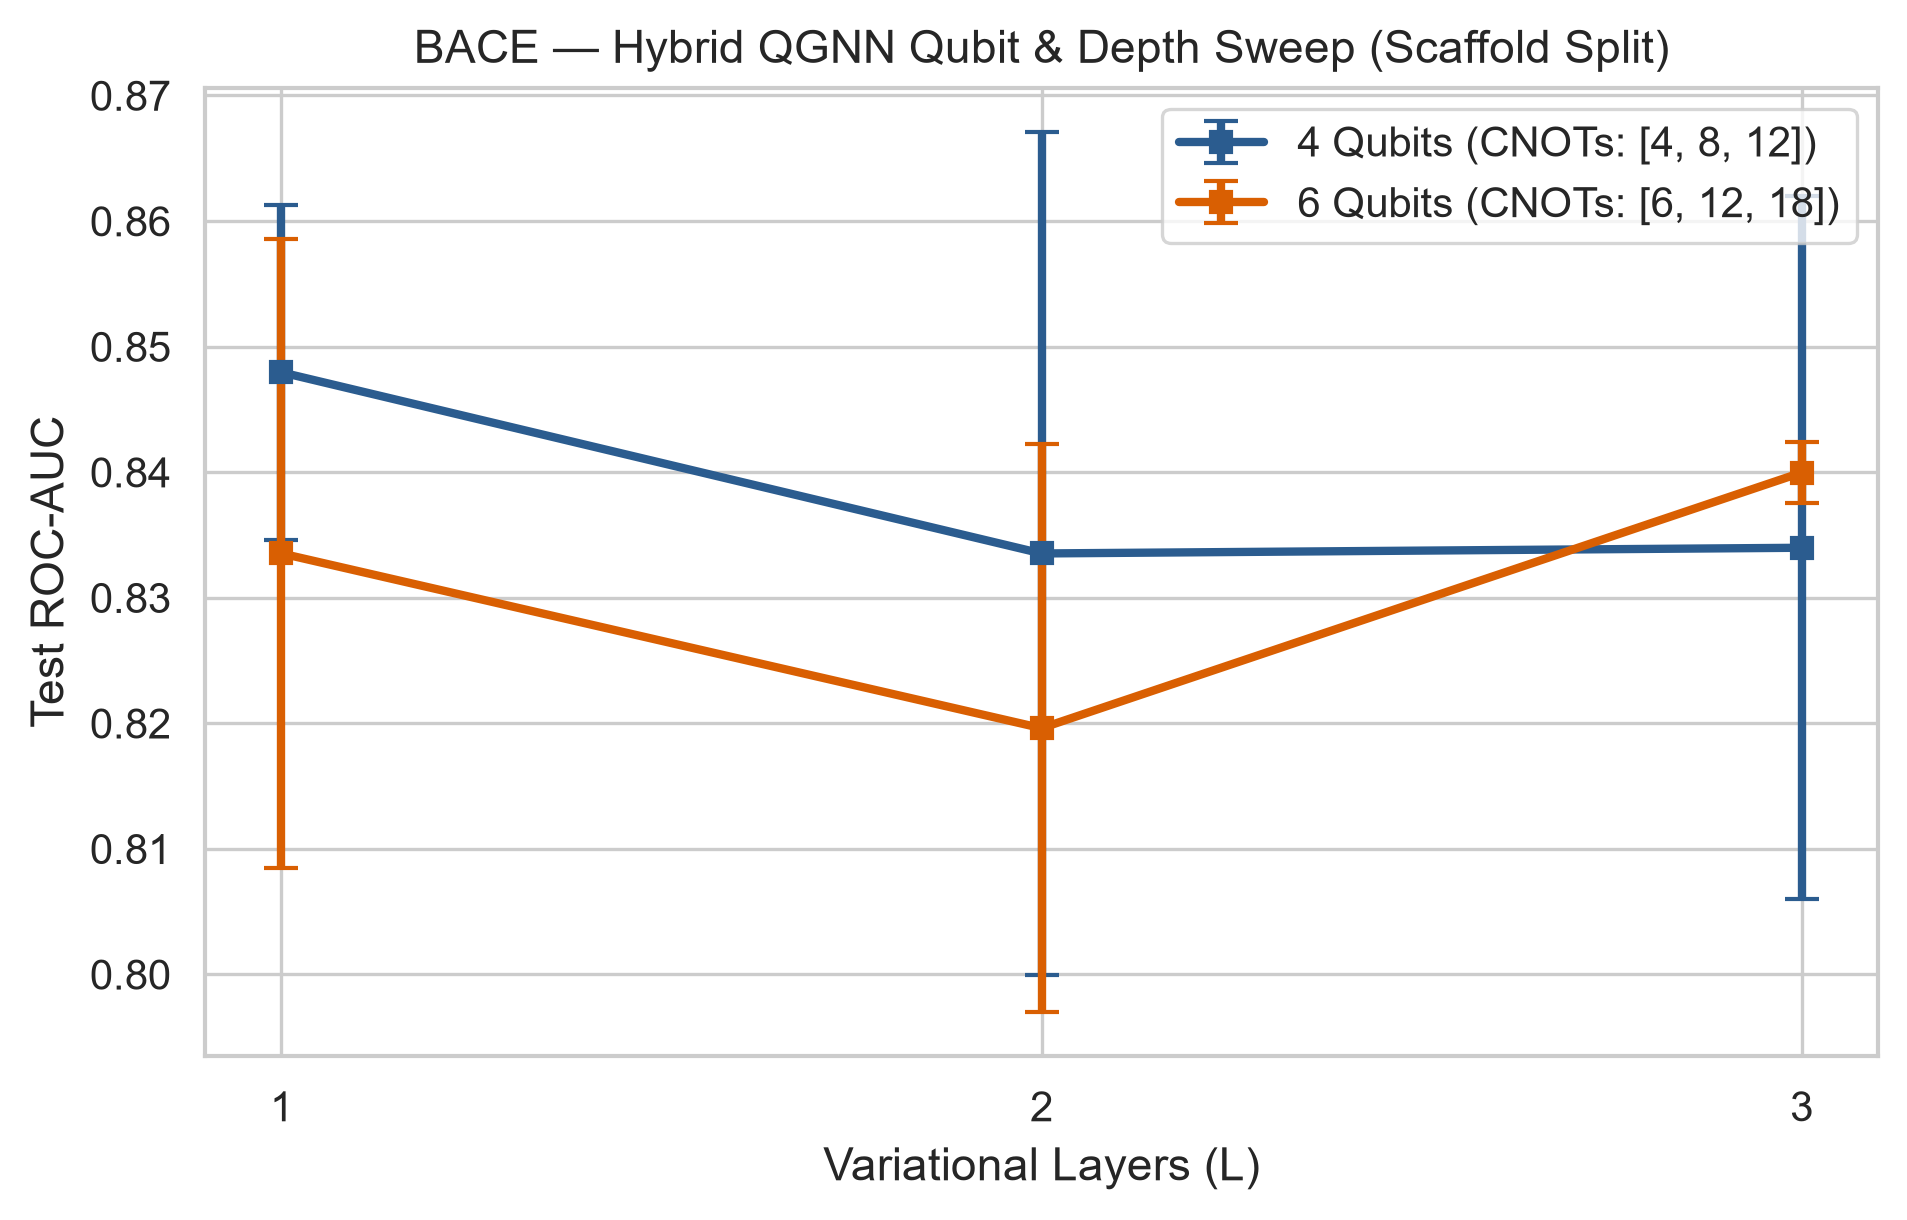
\includegraphics[width=\linewidth]{ablation_qubit_depth.png}
\caption{BACE scaffold-split Test ROC-AUC across 4 and 6 qubits and $L \in \{1,2,3\}$ variational layers.}
\label{fig:qubit_depth}
\end{figure}

\subsection{NISQ Noise Sweep, ZNE Mitigation, and Real IBM QPU Validation}
Table~\ref{tab:nisq} and Fig.~\ref{fig:nisq} show the \texttt{default.mixed} density-matrix sweep across all 152 BACE scaffold test molecules. ZNE reduces Pauli-$Z$ expectation MAE across every non-zero noise level—for example, by $71\%$ at $p=0.005$ ($0.0624 \rightarrow 0.0182$) and $60\%$ at $p=0.010$ ($0.1093 \rightarrow 0.0441$).

\begin{table}[t]
\centering
\caption{NISQ Noise Sweep and ZNE Mitigation (BACE Test, $N=152$)}
\label{tab:nisq}
\begin{tabular}{@{}cccccc@{}}
\toprule
$p_{\text{depol}}$ & $p_{\text{ro}}$ & Unmit. AUC & ZNE AUC & Unmit. MAE & ZNE MAE \\
\midrule
0.000 & 0.00 & 0.8605 & 0.8605 & 0.0000 & 0.0000 \\
0.001 & 0.01 & 0.8607 & 0.8605 & 0.0193 & \textbf{0.0079} \\
0.005 & 0.01 & 0.8611 & 0.8607 & 0.0624 & \textbf{0.0182} \\
0.010 & 0.01 & 0.8611 & 0.8611 & 0.1093 & \textbf{0.0441} \\
0.020 & 0.01 & 0.8627 & 0.8624 & 0.1840 & \textbf{0.1118} \\
0.050 & 0.01 & 0.8642 & 0.8642 & 0.3075 & \textbf{0.2720} \\
\bottomrule
\end{tabular}
\end{table}

\begin{figure}[t]
\centering
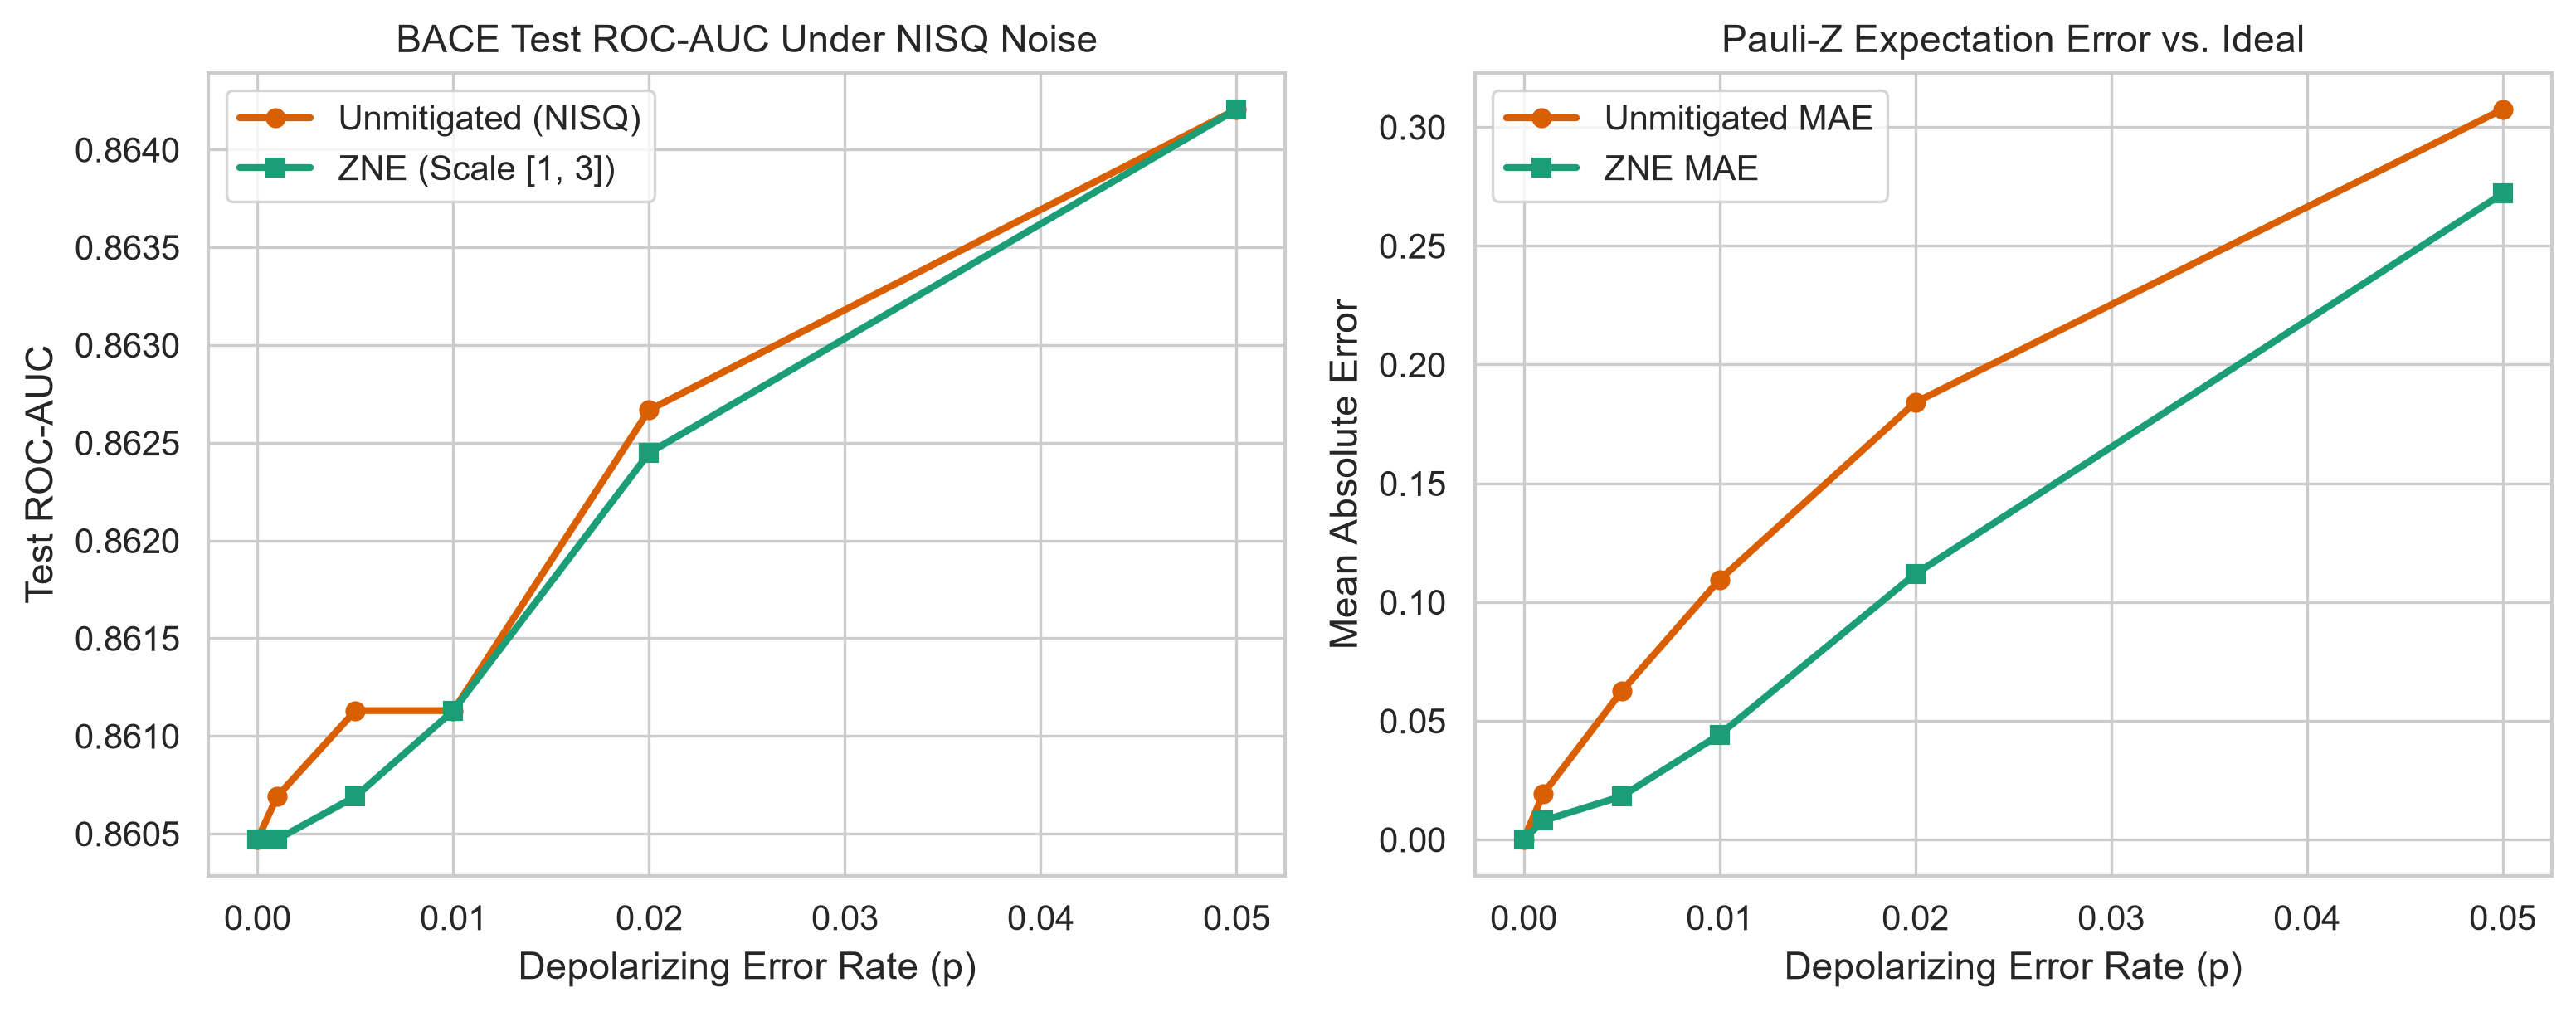
\includegraphics[width=\linewidth]{nisq_noise_zne.png}
\caption{BACE Test ROC-AUC and Pauli-$Z$ MAE under depolarizing + readout noise, comparing unmitigated and ZNE-mitigated inference.}
\label{fig:nisq}
\end{figure}

On real IBM Quantum hardware (\texttt{ibm\_fez}, Job ID \texttt{dc3q0pls2omc738e1m2g}, transpiled depth $71$, $21$ two-qubit gates, $1{,}024$ shots, $N=50$ stratified BACE test molecules), the Hybrid QGNN achieved \textbf{0.8981 ROC-AUC} ($0.7193$ PR-AUC) compared to \textbf{0.9002 ROC-AUC} ($0.7348$ PR-AUC) on the ideal simulator, with $\text{MAE}(\langle Z\rangle) = 0.0677$ and $\text{MAE}(P) = 0.0297$ (Fig.~\ref{fig:ibm_parity}). Fig.~\ref{fig:explainability} shows atom-level gradient saliency maps on unseen BACE and BBBP test scaffolds.

\begin{figure}[t]
\centering
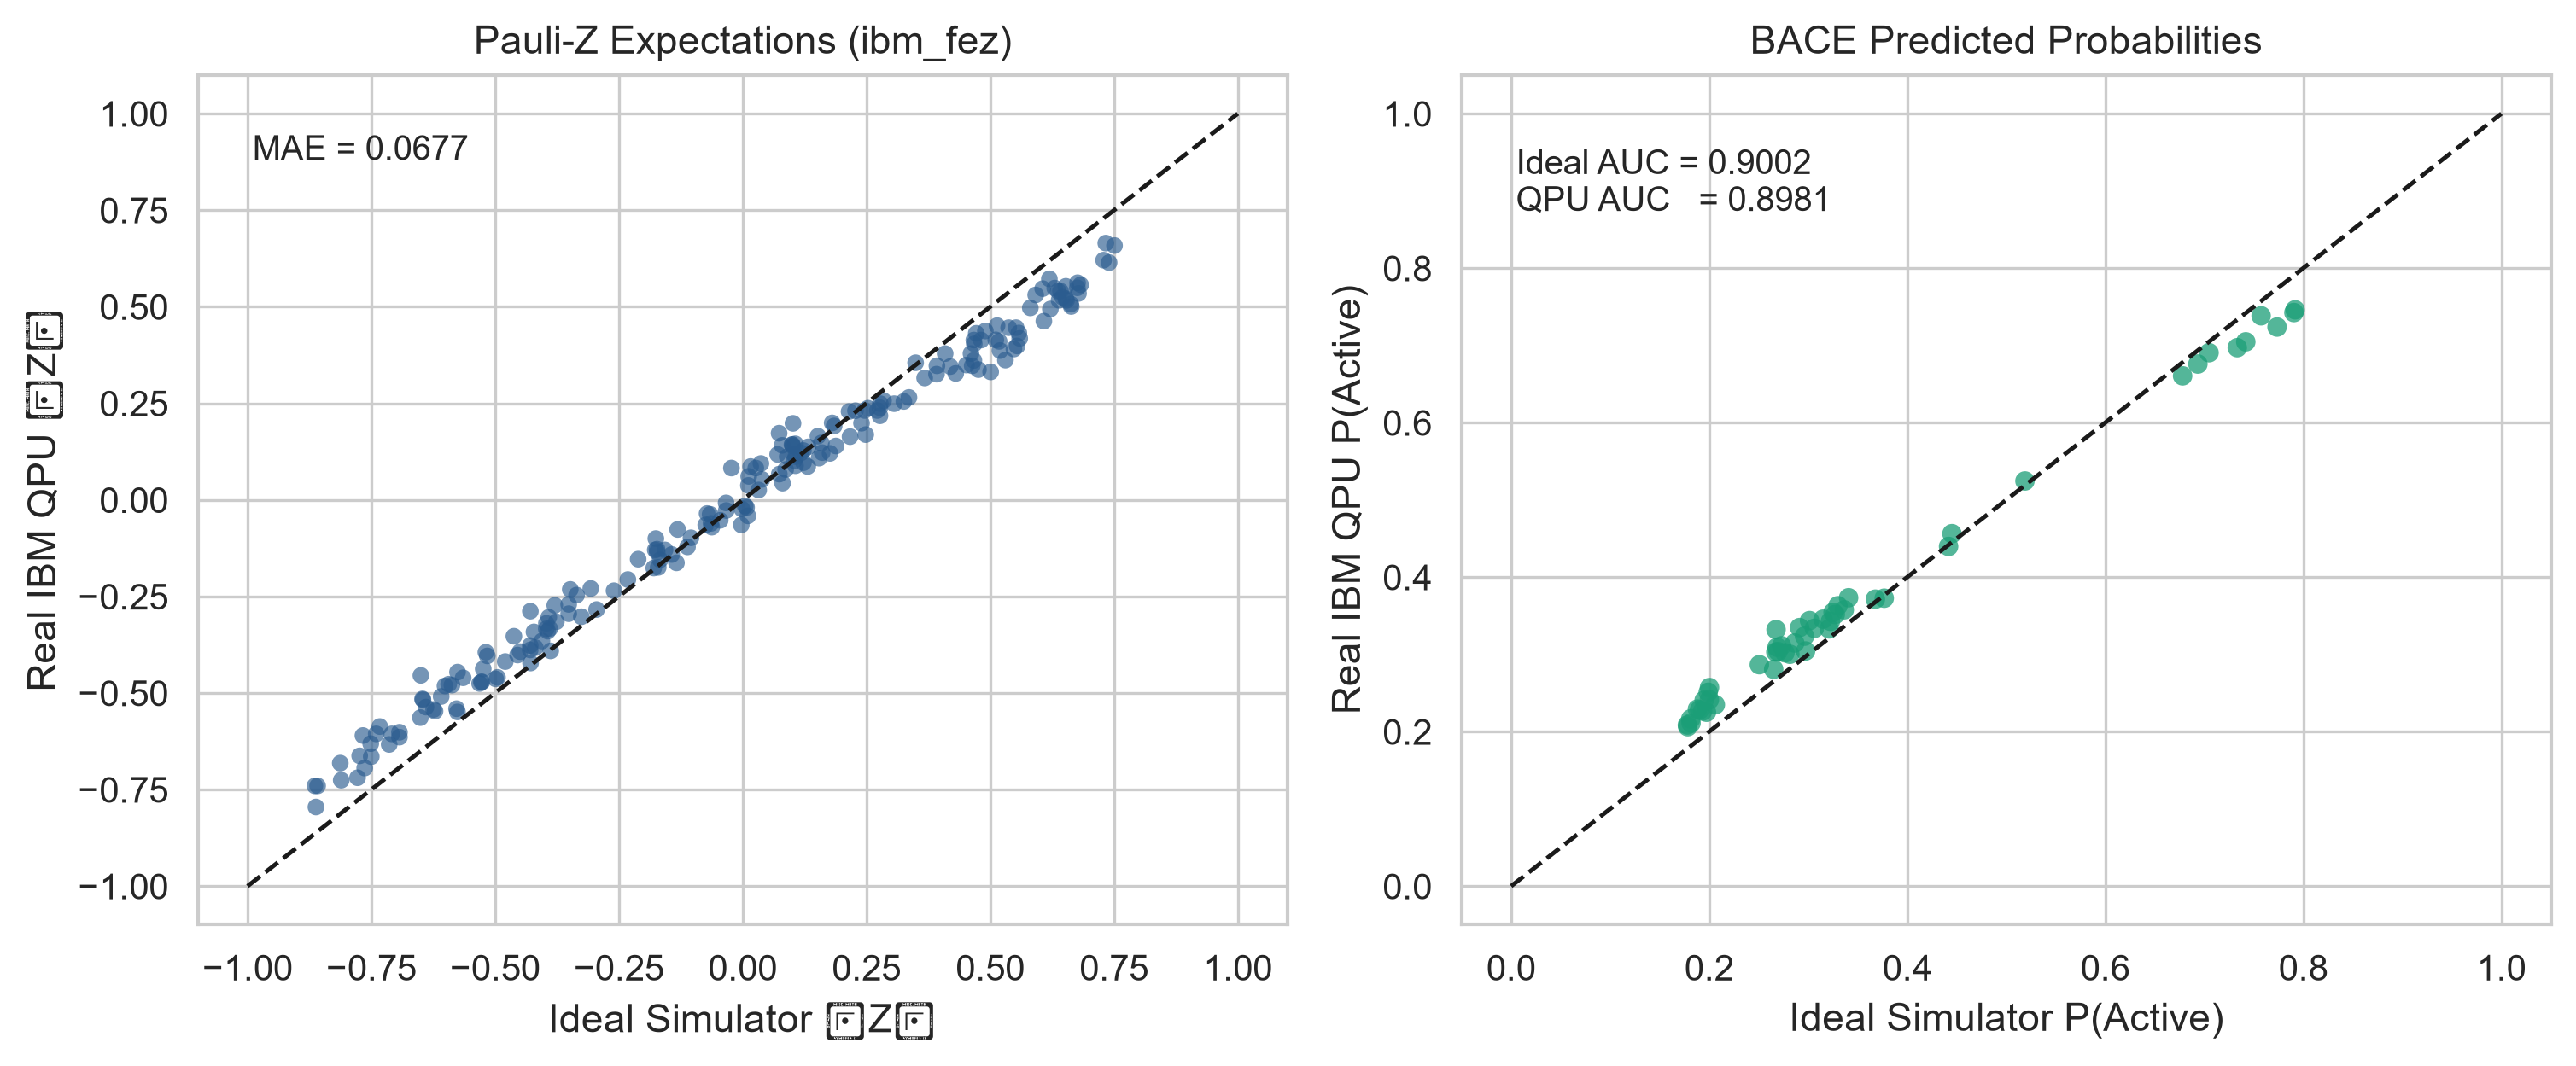
\includegraphics[width=\linewidth]{ibm_qpu_parity.png}
\caption{Parity plot comparing ideal simulation against real \texttt{ibm\_fez} QPU execution ($N=50$ stratified BACE test molecules, Job ID \texttt{dc3q0pls2omc738e1m2g}).}
\label{fig:ibm_parity}
\end{figure}

\begin{figure}[t]
\centering
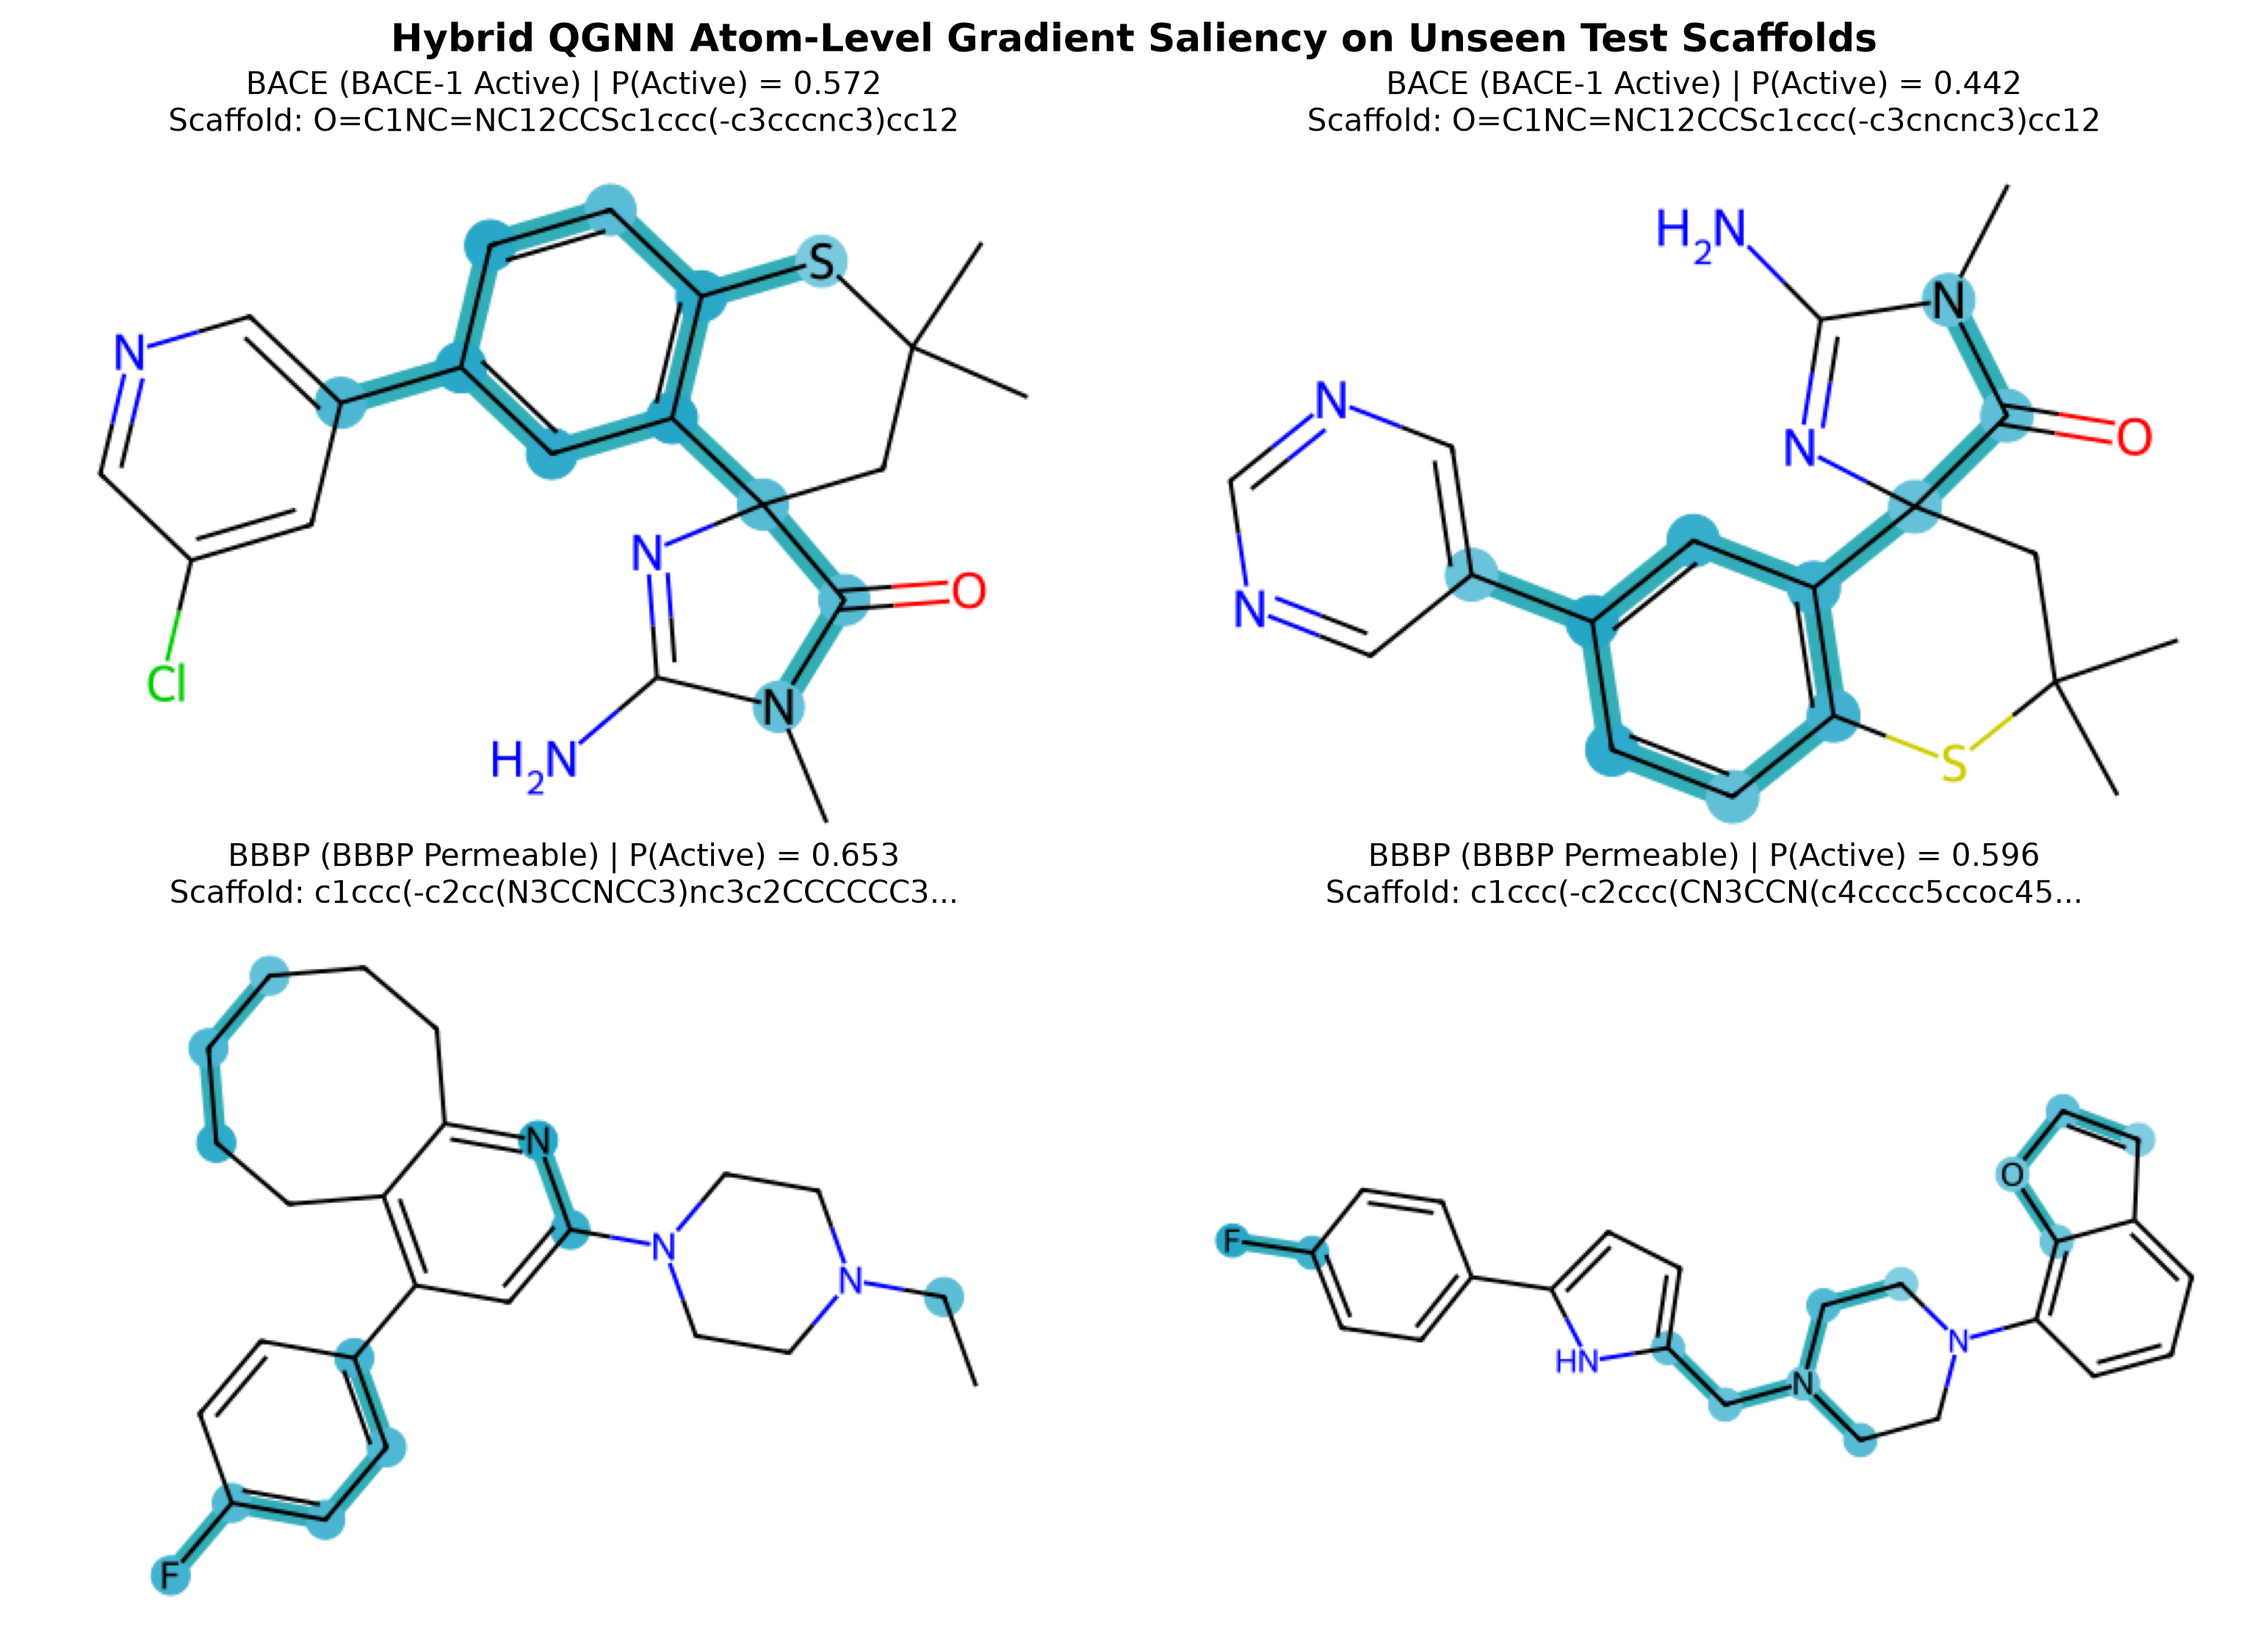
\includegraphics[width=\linewidth]{explainability_substructures.png}
\caption{Atom-level gradient saliency ($\|\partial\,\text{logit}/\partial\,\mathbf{x}_v\|_2$) highlighting pharmacophoric substructures on unseen BACE and BBBP test scaffolds.}
\label{fig:explainability}
\end{figure}

\section{Discussion, Limitations, and Future Work}
\subsection{Why Ranking Metrics Survive Depolarizing Noise}
Notably, Test ROC-AUC remains stable ($0.8605$--$0.8642$) even at $p=0.050$ despite rising expectation MAE ($0.3075$). Global depolarizing noise contracts Bloch vectors isotropically toward the maximally mixed state ($\langle Z_i \rangle \mapsto (1-\lambda)\langle Z_i \rangle$), which scales the linear classifier logits monotonically without altering their rank order—a favorable property for ROC-AUC screening, though probability calibration still requires ZNE.

\subsection{Dataset Trade-offs and NISQ Constraints}
While \texttt{hybrid\_angle} matches \texttt{classical\_matched} on BACE ($0.8340$ vs.\ $0.8360$) and achieves superior PR-AUC ($0.7455$), it trails on BBBP ROC-AUC ($0.6928$ vs.\ $0.7479$), and \texttt{hybrid\_reuploading} exhibits higher multi-seed variance due to steeper periodic loss landscapes. Furthermore, our 4--6 qubit PQC acts as a quantum readout over a 42,500-parameter classical GNN; scaling to larger qubit counts risks barren plateaus \cite{mcclean2018barren} unless paired with local cost functions and shallow hardware-efficient ans\"{a}tze (as supported by our $4q \times 1L$ result of $0.8479$).

\section{Conclusion}
We presented a rigorous, reproducible Hybrid QGNN benchmark for ADMET screening under strict Bemis--Murcko scaffold splitting. By enforcing an exact 41-parameter head comparison, quantifying random-split leakage ($+0.1921$ ROC-AUC inflation on BBBP), demonstrating $59\%$--$71\%$ expectation MAE reduction via ZNE, and validating end-to-end inference on IBM's \texttt{ibm\_fez} QPU ($0.8981$ vs.\ $0.9002$ ideal ROC-AUC), this work establishes a transparent baseline for NISQ-era molecular property prediction.

\bibliographystyle{IEEEtran}
\bibliography{references}

\end{document}
